\documentclass[12pt]{article}
\usepackage{graphicx}
\usepackage{listings}
\usepackage{color}
\usepackage{calc}
\usepackage{setspace}
\usepackage[hidelinks]{hyperref}
\usepackage[dvipsnames]{xcolor}
\usepackage{ragged2e}
\usepackage{geometry}
\usepackage{url}
\usepackage{bm}
\usepackage{amssymb}
\usepackage{amsmath}
\usepackage[indent=0pt]{parskip}

\geometry{
    a4paper,
    left=3cm,
    right=3cm,
    top=3cm,
    bottom=3cm
}

\graphicspath{ {./images/} }
\setlength\parindent{12pt}
\colorlet{Special}{Turquoise!20!MidnightBlue!90!black}
\colorlet{Comment}{Gray!80!black}

% \urldef{\example}\url{https://www.intel.com/content/www/us/en/developer/articles/technical/advanced-encryption-standard-instructions-aes-ni.html}
\begin{document}

\author{Silvio d'Antonio 2145048\\ Riccardo Mearelli 1807331 \\Carlo Segreto 2168340}
\title{Visual Analytics of Italian road accidents\medbreak \normalsize A Visual Analytics project}
\date{A.A. 2025/2026}
\maketitle
\newpage
\tableofcontents
\newpage

\section{Introduction}
\newpage

\section{Background and related work}
\newpage

\section{Visual analytics solution adopted}
\newpage

\section{Discovered insights}
\newpage

\section{References}
\newpage

% Immagine centrata senza didascalia
% \begin{center}
%     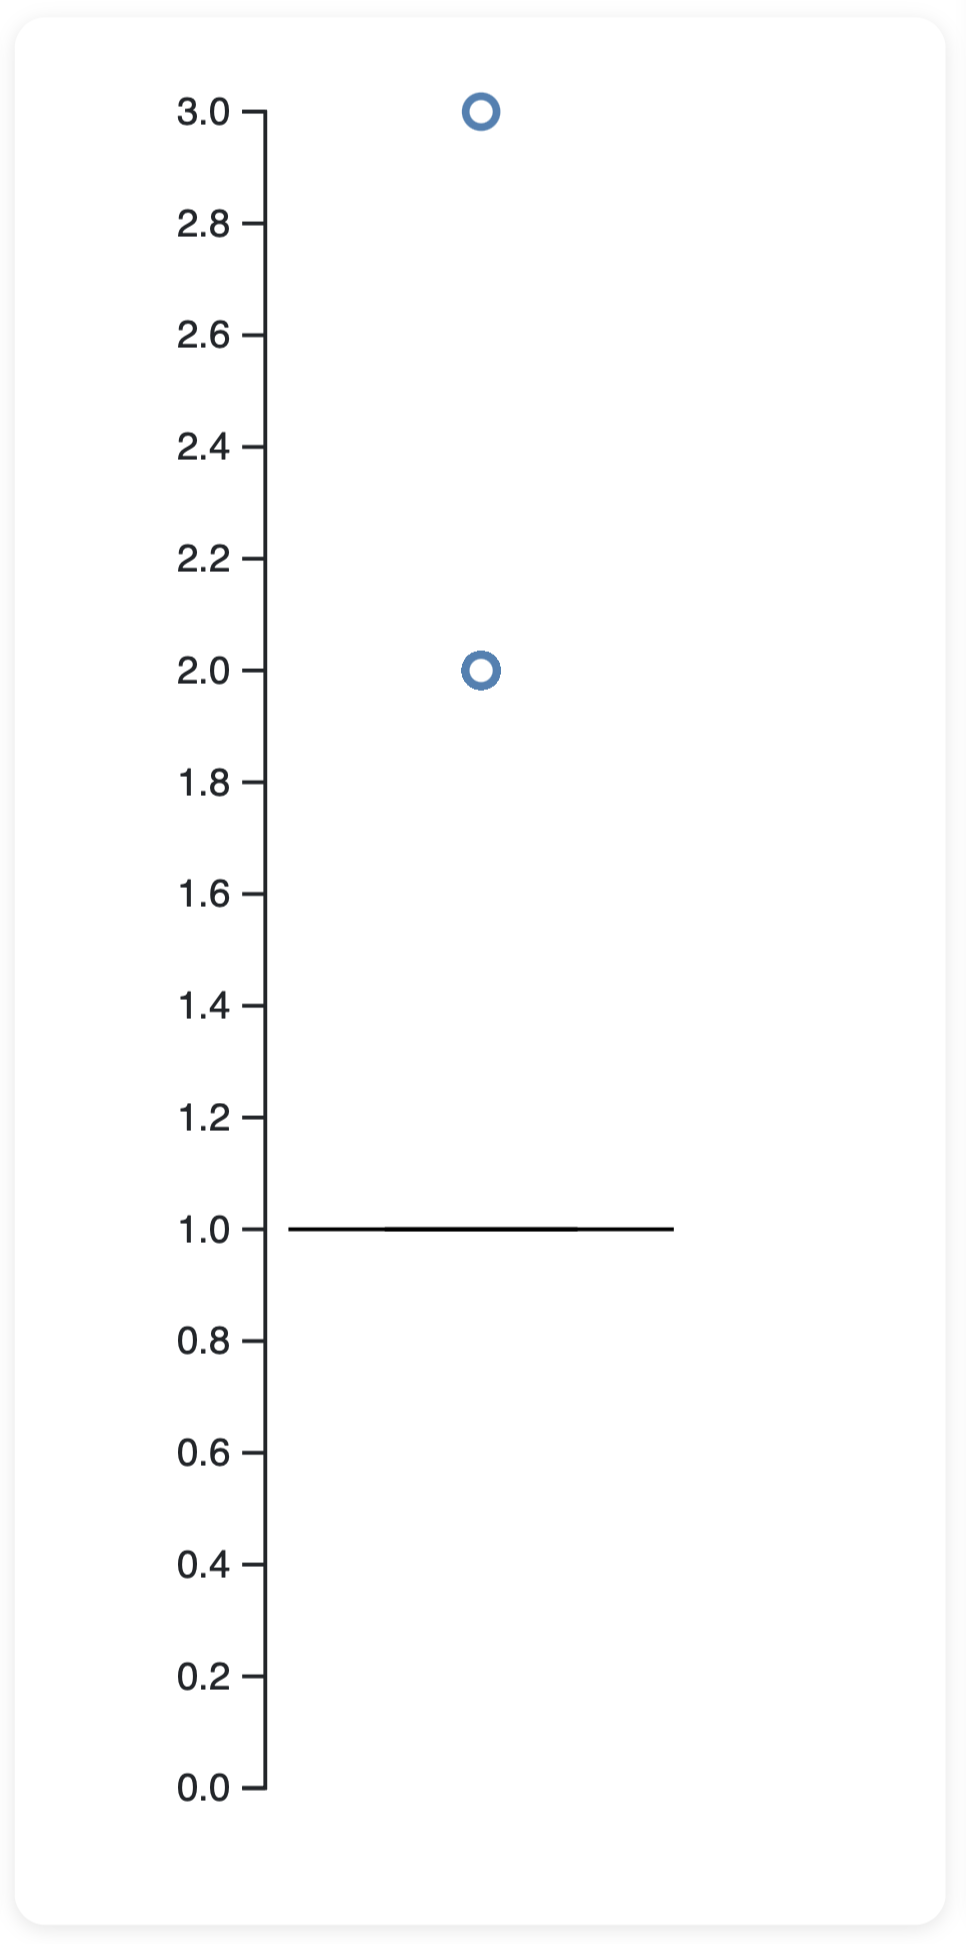
\includegraphics[width=.9\textwidth]{example}
% \end{center}
%\textcolor{Special}{Special colored text}}

% Immagine centrata con didascalia
% \begin{figure}[H]
%     \centering
%     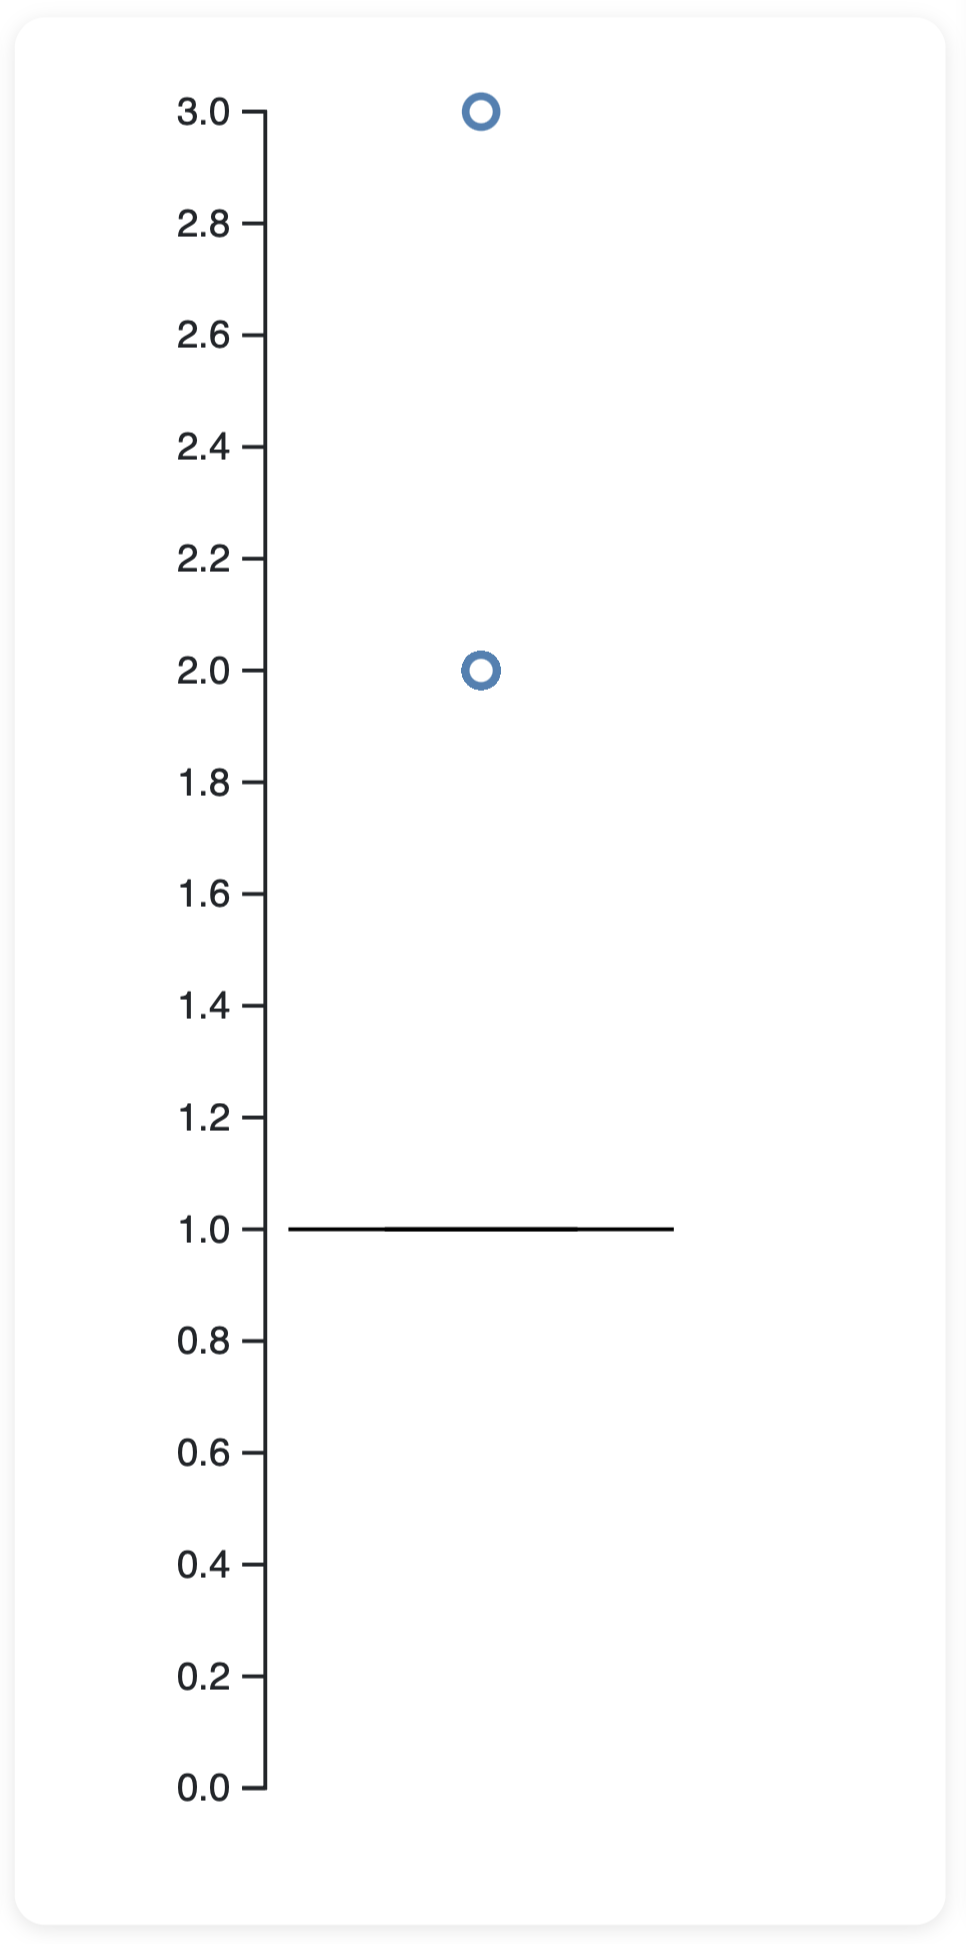
\includegraphics[width=0.5\linewidth]{example}
%     \caption{Example of image insertion.}
% \end{figure}

% Immagine centrata con diascalia per reference
% \begin{figure}[H]
%     \centering
%     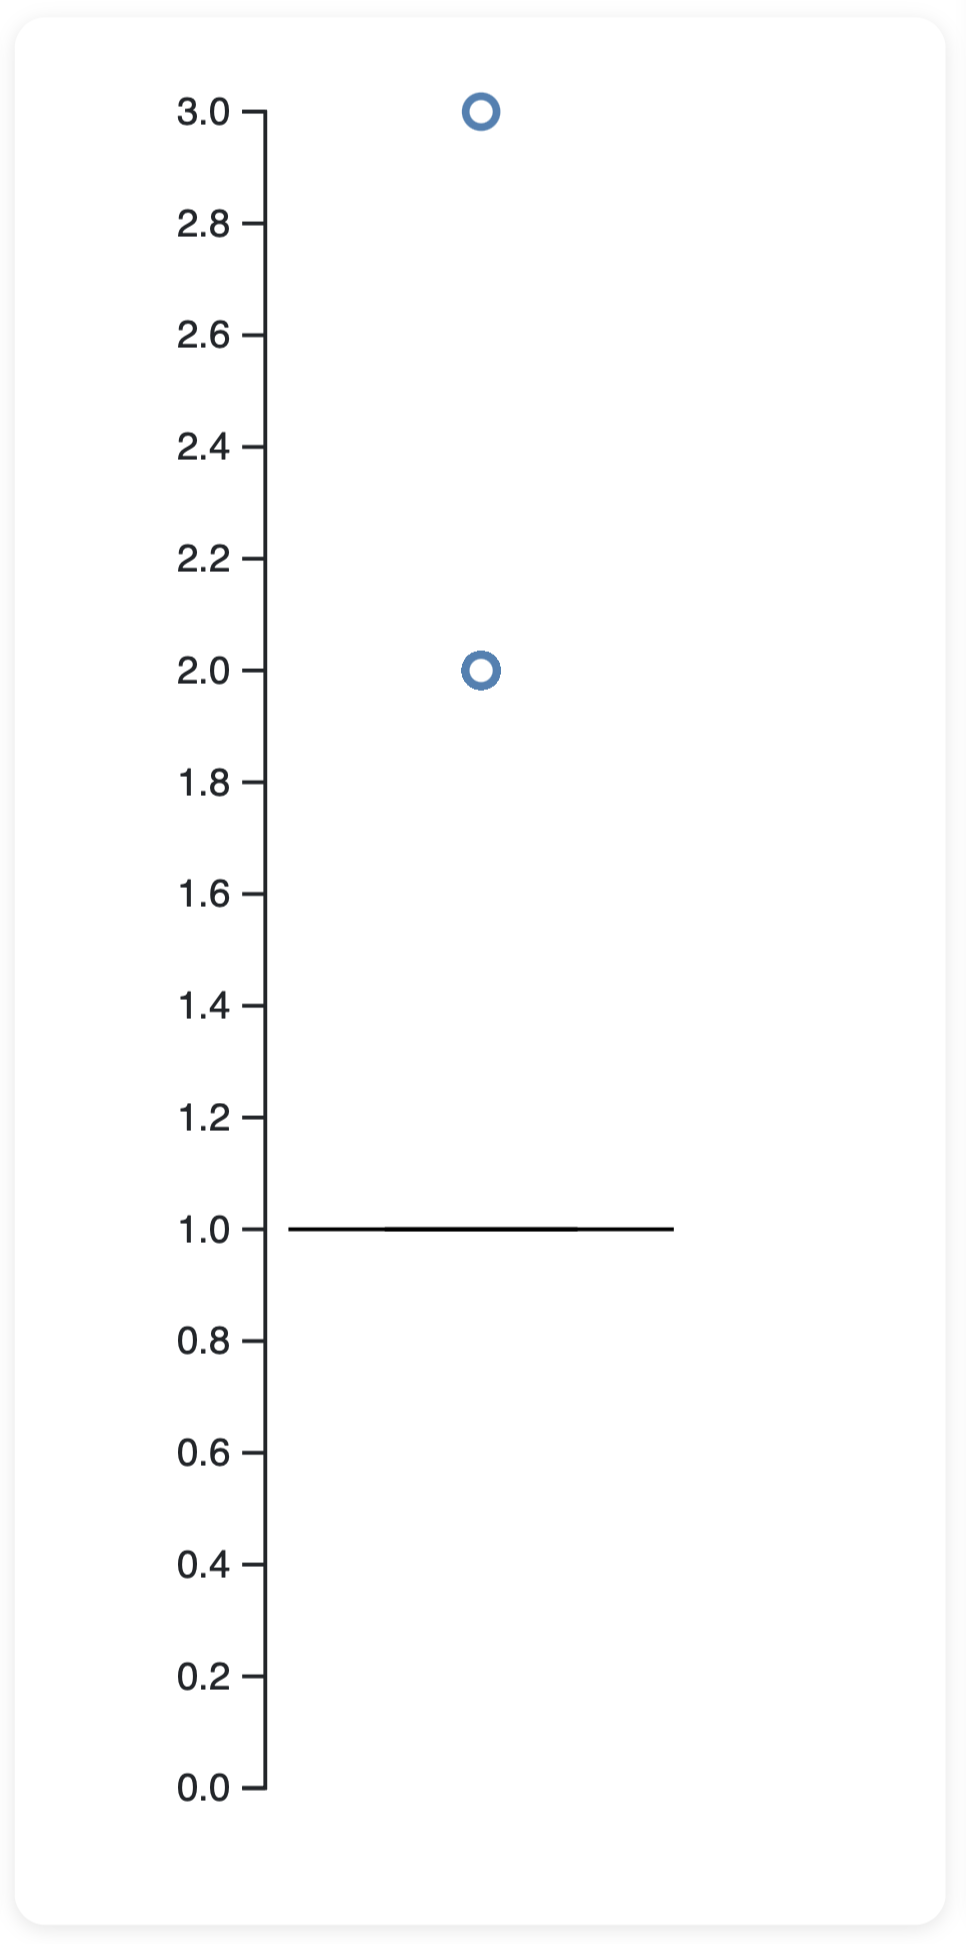
\includegraphics[width=0.5\linewidth]{example}
%     \caption{Example of image insertion.}
%     \label{fig:draft}
% \end{figure}
\end{document}